%!TEX root = ../../main.tex

\chapter{Das dritte Kapitel}
Dies ist der Text des ersten Kapitels.Nur erwähnte Literaturverweise werden auch im Literaturverzeichnis gedruckt: \cite[S.12 ff]{baumgartner:2002}, \cite[S.1-3]{dreyfus:1980}

Meine erste Fußnote\footnote{Ich bin eine Fußnote} darf auch nicht fehlen. Fußnoten sind dazu da, dass man Begriffe näher erklärt, die aber dem vertrauten Leser wahrscheinlich eh bekannt sind. 

\begin{figure}[h]
\centering
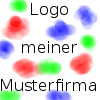
\includegraphics[height=.8\textwidth]{logo.png}
\caption{Das Logo der Musterfirma\footnotemark}
\end{figure}



%\begin{wrapfigure}{r}{.4\textwidth}
%\centering
%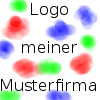
\includegraphics[height=.35\textwidth]{logo.png}
%\vspace{-15pt}
%\caption{Das Logo der Musterfirma\footnotemark}
%\end{wrapfigure}
%Quelle muss in Fußnote stehen (da sonst aufgrund eines Fehlers nicht kompiliert
% wird)
\footnotetext{aus \cite{mustermann:2012}}
Looking for the one superhero comic you just have to read. Following the antics and adventures of May Mayday Parker, this Spider-book has everything you could want in a comic--action, laughs, mystery and someone in a Spidey suit. Collects Alias \#1-28, What If. Jessica Jones had Joined the Avengers. In her inaugural arc, Jessicas life immediately becomes expendable when she uncovers the potentially explosive secret of one heros true identity. In her inaugural arc, Jessicas life immediately becomes expendable when she uncovers the potentially explosive secret of one heros true identity.

Manchmal braucht man auch Formeln. LaTeX hat einen sehr guten Formeleditor, der eigentlich selbsterklärend ist. Die Formeln weden automatisch nummeriert, aber man kann immer im Text mit einem Label wie Formel \ref{xyz} Bezug nehmen.

\begin{equation}
t-t_{0}=\sqrt{\frac{l}{g}}\int_{0}^{\varphi}{\frac{d\psi}{\sqrt{1-k^{2}\sin^{2} {\psi}}}} = \sqrt{\frac{l}{g}} F(k,\varphi)
\label{xyz}
\end{equation}

Manchmal braucht man Aufzählungen, die man in einzelnenen Punkten aufführt.
\begin{itemize}
\item Dies ist der erste Punkt, der aufgeführt wird.
\item Dies ist der zweite Punkt, der aufgeführt wird. Manchmal will man auch etwas \textbf{fett} oder \textit{kursiv} oder \textbf{\textit{beides in Kombination}}  drucken.
\item Dies ist der dritte Punkt, der aufgeführt wird.
\end{itemize}

Once upon a time, Jessica Jones was a costumed super-hero, just not a very good one. First, a story where Wolverine and Hulk come together, and then Captain America and Cable meet up. In a city of Marvels, Jessica Jones never found her niche. The classic adventures of Spider-Man from the early days up until the 90s. Looking for the one superhero comic you just have to read. In her inaugural arc, Jessicas life immediately becomes expendable when she uncovers the potentially explosive secret of one heros true identity.

Erste Erwähnung eines Akronyms wird als Fußnote angezeigt. Jede weitere wird
nur verlinkt: \acf{AGPL}. \cite{fsf:2007}

Verweise auf das Glossar: \gls{Glossareintrag}, \glspl{Glossareintrag}

